%% description of the retrieval method and the evaluation using various
%% ground-based observations

%% Copernicus Publications Manuscript Preparation Template for LaTeX Submissions
%% ---------------------------------
%% This template should be used for copernicus.cls
%% The class file and some style files are bundled in the Copernicus Latex Package which can be downloaded from the different journal webpages.
%% For further assistance please contact the Copernicus Publications at: publications@copernicus.org
%% http://publications.copernicus.org


%% Please use the following documentclass and Journal Abbreviations for Discussion Papers and Final Revised Papers.


%% 2-Column Papers and Discussion Papers
\documentclass[essd,manuscript]{copernicus}\usepackage[]{graphicx}\usepackage[]{color}
%% maxwidth is the original width if it is less than linewidth
%% otherwise use linewidth (to make sure the graphics do not exceed the margin)
\makeatletter
\def\maxwidth{ %
  \ifdim\Gin@nat@width>\linewidth
    \linewidth
  \else
    \Gin@nat@width
  \fi
}
\makeatother

\definecolor{fgcolor}{rgb}{0.345, 0.345, 0.345}
\newcommand{\hlnum}[1]{\textcolor[rgb]{0.686,0.059,0.569}{#1}}%
\newcommand{\hlstr}[1]{\textcolor[rgb]{0.192,0.494,0.8}{#1}}%
\newcommand{\hlcom}[1]{\textcolor[rgb]{0.678,0.584,0.686}{\textit{#1}}}%
\newcommand{\hlopt}[1]{\textcolor[rgb]{0,0,0}{#1}}%
\newcommand{\hlstd}[1]{\textcolor[rgb]{0.345,0.345,0.345}{#1}}%
\newcommand{\hlkwa}[1]{\textcolor[rgb]{0.161,0.373,0.58}{\textbf{#1}}}%
\newcommand{\hlkwb}[1]{\textcolor[rgb]{0.69,0.353,0.396}{#1}}%
\newcommand{\hlkwc}[1]{\textcolor[rgb]{0.333,0.667,0.333}{#1}}%
\newcommand{\hlkwd}[1]{\textcolor[rgb]{0.737,0.353,0.396}{\textbf{#1}}}%
\let\hlipl\hlkwb

\usepackage{framed}
\makeatletter
\newenvironment{kframe}{%
 \def\at@end@of@kframe{}%
 \ifinner\ifhmode%
  \def\at@end@of@kframe{\end{minipage}}%
  \begin{minipage}{\columnwidth}%
 \fi\fi%
 \def\FrameCommand##1{\hskip\@totalleftmargin \hskip-\fboxsep
 \colorbox{shadecolor}{##1}\hskip-\fboxsep
     % There is no \\@totalrightmargin, so:
     \hskip-\linewidth \hskip-\@totalleftmargin \hskip\columnwidth}%
 \MakeFramed {\advance\hsize-\width
   \@totalleftmargin\z@ \linewidth\hsize
   \@setminipage}}%
 {\par\unskip\endMakeFramed%
 \at@end@of@kframe}
\makeatother

\definecolor{shadecolor}{rgb}{.97, .97, .97}
\definecolor{messagecolor}{rgb}{0, 0, 0}
\definecolor{warningcolor}{rgb}{1, 0, 1}
\definecolor{errorcolor}{rgb}{1, 0, 0}
\newenvironment{knitrout}{}{} % an empty environment to be redefined in TeX

\usepackage{alltt}



%% Journal Abbreviations (Please use the same for Discussion Papers and Final Revised Papers)

% Archives Animal Breeding (aab)
% Atmospheric Chemistry and Physics (acp)
% Advances in Geosciences (adgeo)
% Advances in Statistical Climatology, Meteorology and Oceanography (ascmo)
% Annales Geophysicae (angeo)
% ASTRA Proceedings (ap)
% Atmospheric Measurement Techniques (amt)
% Advances in Radio Science (ars)
% Advances in Science and Research (asr)
% Biogeosciences (bg)
% Climate of the Past (cp)
% Drinking Water Engineering and Science (dwes)
% Earth System Dynamics (esd)
% Earth Surface Dynamics (esurf)
% Earth System Science Data (essd)
% Fossil Record (fr)
% Geographica Helvetica (gh)
% Geoscientific Instrumentation, Methods and Data Systems (gi)
% Geoscientific Model Development (gmd)
% Geothermal Energy Science (gtes)
% Hydrology and Earth System Sciences (hess)
% History of Geo- and Space Sciences (hgss)
% Journal of Sensors and Sensor Systems (jsss)
% Mechanical Sciences (ms)
% Natural Hazards and Earth System Sciences (nhess)
% Nonlinear Processes in Geophysics (npg)
% Ocean Science (os)
% Proceedings of the International Association of Hydrological Sciences (piahs)
% Primate Biology (pb)
% Scientific Drilling (sd)
% SOIL (soil)
% Solid Earth (se)
% The Cryosphere (tc)
% Web Ecology (we)



%% \usepackage commands included in the copernicus.cls:
%\usepackage[german, english]{babel}
%\usepackage{tabularx}
%\usepackage{cancel}
%\usepackage{multirow}
%\usepackage{supertabular}
%\usepackage{algorithmic}
%\usepackage{algorithm}
%\usepackage{amsthm}
%\usepackage{float}
%\usepackage{subfig}
%\usepackage{rotating}
\usepackage{mathptmx}
%% \usepackage[T1]{fontenc}

\newcommand\comment[2]{\{\hlnum{ \textit{#1}: #2}\}}
\newcommand\commentjm[1]{\comment{$j_\mu$}{#1}}
\IfFileExists{upquote.sty}{\usepackage{upquote}}{}
\begin{document}



%% \linenumbers

\title{Using CALIOP to estimate cloud-field base height and its uncertainty}


% \Author[affil]{given_name}{surname}

\Author[1]{Johannes}{M\"ulmenst\"adt}
\Author[1]{Odran}{Sourdeval}
\Author[2]{Tristan S.}{L'Ecuyer}
\Author[3]{Christoph}{B\"ohm}
%%\Author[1]{Edward}{Gryspeerdt}
\Author[1]{Johannes}{Quaas}

\affil[1]{Institute of Meteorology, Universit\"at Leipzig, Leipzig, Germany}
\affil[2]{University of Wisconsin, Madison, USA}
\affil[3]{Institute for Geophysics and Meteorology, Universit\"at zu K\"oln, K\"oln, Germany}

%% The [] brackets identify the author with the corresponding affiliation. 1, 2, 3, etc. should be inserted.



\runningtitle{Cloud base heights from CALIOP}

\runningauthor{M\"ulmenst\"adt et al.}

\correspondence{Johannes M\"ulmenst\"adt
  (\href{mailto:johannes.muelmenstaedt@uni-leipzig.de}{johannes.muelmenstaedt@uni-leipzig.de})}



\received{}
\pubdiscuss{} %% only important for two-stage journals
\revised{}
\accepted{}
\published{}

%% These dates will be inserted by Copernicus Publications during the typesetting process.


\firstpage{1}

\maketitle



\begin{abstract}
  A technique is presented that uses attenuated backscatter profiles
  from the CALIOP satellite lidar to estimate cloud base heights.  Even when
  clouds are thick enough to attenuate the lidar beam (optical thickness
  $\tau \gtrsim 5$), the technique provides cloud base heights by treating the
  cloud base height of nearby thinner clouds as representative of the
  surrounding cloud field.  Using ground-based ceilometer data, uncertainty
  estimates for the cloud base height product at retrieval resolution are
  derived as a function of various properties of the CALIOP lidar profiles.
  Evaluation of the predicted cloud base heights and their predicted uncertainty
  using a second, statistically independent, ceilometer dataset shows that cloud
  base heights and uncertainties are biased by less than 10\%.  Geographic
  distributions of cloud base height and its uncertainty are presented.
  Regionally, the uncertainty is found to be substantially smaller than the
  480~m uncertainty assumed in the A-Train downwelling longwave estimate,
  potentially permitting the most uncertain of the radiative fluxes in the
  climate system to be better constrained.
\end{abstract}

\introduction  %% \introduction[modified heading if necessary]
\label{sec:intro}
Cloud base height (CBH) is an important geometric parameter of a cloud.  It
controls how much downwelling longwave radiation the cloud emits.  Aerosol
concentration and updraft speed at that level determine the microphysical
characteristics of the cloud.  It is one of the parameters that is required in
the calculation of the subadiabaticity of the cloud.  However, due to the
viewing geometry, it is also one of the most difficult cloud parameters to
retrieve from satellite.

Multiple methods have been proposed for satellite determination of the cloud
base height.  \cite{Zhu2014} have used the Visible Infrared Imaging Radiometer Suite
aboard the Suomi National Polar-orbiting Partnership satellite
\citep[VIIRS,][]{Cao2014} to estimate cloud base temperature (CBT) from the
lowest cloud-top temperature within a cloud cluster; a reanalysis temperature
profile can be used to convert CBT to CBH.  Using an empirical relationship
between geometric and optical thickness, \cite{Fitch2016} have obtained CBH from
VIIRS.  Cloud geometric thickness (and therefore CBH if the cloud top height is
known) can be inferred from increased spectral absorption by O$_2$ within cloud
due to multiple scattering \citep{Kokhanovsky2005}.  Stereoscopic determination of
the height of the most reflective layer \citep{Naud2005,Naud2007} in Multiangle
Imaging Spectroradiometer data \citep[MISR,][]{Diner1998} yields information on
CBH, as the lowest layer heights within a cloud cluster may correspond to the
base of a cloud seen from its side.  An evaluation of MISR
  techniques is in progress \citep{Boehm2017}.

For analyses wishing to combine cloud base information with other cloud
properties retrieved by A-Train satellites, these methods share the disadvantage
that the required instruments are not part of the A-Train.  Methods that are
applicable to A-Train satellites are based on Moderate Resolution Imaging
Spectroradiometer \citep[MODIS,][]{Platnick2017} cloud properties retrieved near
cloud top and integrated along moist adiabats to determine the cloud thickness
\citep{Meerkoetter2007} or on active remote sensing by CloudSat
\citep[2B-GEOPROF,][]{Marchand2008} or a combination of CloudSat and CALIOP
\citep[2B-GEOPROF-LIDAR,][]{Mace2014}.  Each of these has drawbacks.  The
MODIS-derived cloud thickness assumes adiabatic cloud profiles and therefore
cannot be used to constrain subadiabaticity; the use of ancillary temperature
profile estimates may also be problematic in many cases.  CloudSat misses the
small droplets at the base of nonprecipitating clouds, and retrievals are
further degraded in the ground clutter region.  CALIOP detects the bases of only
the thinnest clouds \citep[$\tau < 5$,][]{Mace2014}; frequently, it is desirable
to know the base height of thick clouds as well.

In this paper, we revisit the CALIOP cloud base determination.  This relies on
one central assumption, namely that, because the
lifting condensation level is approximately homogeneous within an airmass, the
cloud bases retrieved by CALIOP for thin clouds may be a good proxy for the cloud
base heights of an entire cloud field, including the optically thicker clouds
within the field.  
We have designed an algorithm that extrapolates the CALIOP
cloud-base measurements into locations where CALIOP attenuates before reaching
cloud base.  This algorithm is called CBASE (Cloud Base Altitude Spatial
Extrapolator).  In this paper we evaluate its performance by comparing CBASE
CBH against CBH observed by ground-based
ceilometers.

The cloud base of interest in this analysis is the base of the lowest cloud in
each column. Even if it CALIOP can also detect the base heights of other layers
in multilayer situations, it is the base height of the lowest cloud that is of
largest interest for many applications (e.g., surface radiation
estimates). 

Section~\ref{sec:data} describes the data sources used in determining and
evaluating CBH.  In Section~\ref{sec:algorithm} we describe
the algorithm and evaluate its performance, including error statistics.  The
publicly available processed CBASE output is described in
Section~\ref{sec:results}.  We conclude in Section~\ref{sec:conclusions} with an
outlook on the longstanding questions that the CBASE dataset can address.

\section{Data}
\label{sec:data}

Two classes of data are used in this work: cloud lidar data, from which we
intend to derive a global CBH dataset; and ground-based observations used as
reference measurements of CBH to train and evaluate the algorithm by which
CBH is determined from the satellite data.

\subsection{CALIOP VFM}

The input satellite data to our analysis is from the Cloud-Aerosol Lidar with
Orthogoncal Polarization \cite[CALIOP][]{Winker2007} on board the Cloud-Aerosol Lidar and Infrared Pathfinder
Satellite Observation (CALIPSO) satellite that is part of the A-Train
satellite constellation \citep{Stephens2002} on a
sun-synchronous low-Earth orbit with equator crossings at approximately 1330 hours local
time. The cloud-base product relies on the retrieved vertical feature mask
\citep[VFM,][]{vaughan2002}.  For each CALIOP lidar backscatter profile, the VFM identifies features
such as clear air, cloud, aerosol, or planetary surface; this is termed the ``feature
type''.  (When the lidar beam is completely attenuated, this is reported as a
feature type.)  In addition to the feature type, the VFM records the degree of
confidence in the identification (``none'' to ``high'', termed the ``feature
type QA flag''); the thermodynamic phase of a layer identified as cloud as well
as the degree of confidence therein (termed ``ice water phase'' and ``ice water
phase QA flag''); the horizontal distance over which the algorithm had to
average to identify a feature above noise and molecular atmospheric scattering
(``horizontal averaging distance'').  

In the present analysis, we use VFM version 4.10 \citep{vfm}, the current
``standard'' release, for the years 2007 and 2008.  The VFM files are obtained
from ICARE \citep{icare}.
% \commentjm{Citation: CALIPSO Science Team (2016), CALIPSO/CALIOP Level 2,
%   Vertical Feature Mask Data, version 4.10, Hampton, VA, USA: NASA Atmospheric
%   Science Data Center (ASDC), Accessed <author citing data inserts date here> at
%   doi: 10.5067/CALIOP/CALIPSO/LID\_L2\_VFM-Standard-V4-10}

\subsection{Airport ceilometers}





For optimizing several parameters of the algorithm, for determining the expected
cloud base uncertainty, and for evaluation of the trained algorithm, reference
measurements of CBH are required.  The source of these ``true'' CBH in this work
is ground-based cloud observations at airports.  Weather observations at
airports are disseminated worldwide in aviation routine and special weather
reports \citep[METARs and SPECIs, collectively referred to as METARs
henceforth,][]{metar}.  Apart from providing airport weather information for
aviation, METAR data is used for assimilation into numerical weather prediction
(NWP) models \citep[e.g.,][]{Benjamin2016, Dee2011}.  In many locations, CBH
reported in METARs is measured by a ceilometer over a period of time (tens of
minutes) and then objectively grouped into cloud layers and their respective
fractional coverages, using the temporal variation at a fixed point under an
advected cloud field as a proxy for spatial variability of the cloud field
\citep[e.g.,][]{Heese2010}.  METAR data is widely distributed and archived; the
data for the present analysis was downloaded from the Weather Underground
archive \citep{wunderground}.

In the United States, CBH is mostly derived automatically by laser ceilometers
that form part of Automated Surface Observing Stations \citep[ASOS,][]{asos}
system; see, e.g., \cite{An2017,Ikeda2017} for recent examples of ASOS
application to deriving cloud climatologies or NWP model evaluation.  In other
parts of the world, the cloud bases may be estimated by human observers or may
be omitted under certain conditions when the lowest cloud base is higher than
5000~feet, complicating objective comparison to satellite CBH.  To ensure that
the ceilometer CBH are of high and spatially uniform quality, we restrict
ourselves to METARs from the contiguous continental United States.

There are 1645 %
stations throughout the continental USA that lie within 100~km of a CALIOP
footprint.  In normal operation, the time resolution of CBH reports is 1~h, but
during rapidly changing conditions, more frequent updates may be provided; for
comparison to satellite CBH, the ceilometer observation closest in time to the
satellite overpass is used, provided that the time difference is less than 1~h.
For training the algorithm, we use ceilometer observations from the year 2008.
For unbiased evaluation of the algorithm performance, a statistically
independent dataset is required; we use ceilometer observations from the same
stations from the year 2007.  Figure~\ref{fig:asos} shows the locations of these
stations along with the number of satellite--ceilometer CBH coincidences and the
closest co-location distance during the year 2007.

\section{CBASE Algorithm and evaluation}
\label{sec:algorithm}

The CBASE algorithm and evaluation proceed in four steps:
\begin{enumerate}
\item We determine the CBH from all CALIOP profiles where the
  surface generates a return, indicating that the lidar is not completely
  attenuated by cloud.  We refer to this as the \textit{local
    CBH} in the sense that it is local to the CALIOP profile.
\item Using ground-based ceilometer data, we determine quality of cloud base
  height depending on a number of properties of the CALIOP profile.  Assuming
  those properties suffice to determine the quality of the CBH estimate, we
  can then predict the quality of a cloud base as a function of those factors.
  The quality metric we use is the root mean square error (RMSE); the category
  RMSE determined from comparison to ceilometer CBH then serves as the predicted
  CBH uncertainty.  In the language of machine learning, we refer to this step
  as \textit{training} the algorithm on the ceilometer data to predict CBH and
  CBH uncertainty.
\item Based on the predicted quality of each local cloud base, we either reject
  the local cloud base or combine it with other local cloud bases within a
  distance $D_\text{max}$ of the point of interest (POI) to arrive at an 
  estimate of the CBH and its uncertainty at the POI.
\item Using a statistically independent validation dataset, we verify that the
  predicted CBH and its uncertainty are correct.
\end{enumerate}

This section is divided into four subsections, one for each algorithm step
enumerated above.

\subsection{Determination of local CBH}
\label{sec:algorithm:local}
Local CBH is determined from the CALIOP VFM for each profile with a surface
return.  The rationale is that a surface return indicates that the lidar did not
attenuate within the cloud, and that the lower limit of the layer identified as
cloud therefore corresponds to the cloud base; Figure~\ref{fig:method}
illustrates the idea.  For these profiles, the location, CBH, cloud top height,
feature type between the cloud base and the surface,
cloud thermodynamic phase, and associated quality assurance flags from the VFM
algorithm are recorded.

\subsection{Determination of local cloud base quality}
\label{sec:algorithm:qual}
We assess the quality of the CALIOP CBH $z$ using the root mean square error
(RMSE) with respect to the
ceilometer-observed CBH $\hat{z}$.  The RMSE is defined as
\begin{equation}
  \label{eq:rmse}
  E = \sqrt{\frac{1}{N}\sum\limits_{i = 1}^{N}\left(z_i - \hat{z}\right)^2}.
\end{equation}
The sum runs over all CALIOP profiles containing at least one cloud layer and a
surface return that are within 100~km horizontal distance of the ceilometer,
occurred within 3600~s of a ceilometer observation, and have their lowest CALIOP
cloud feature within 3~km of the surface.  Ceilometer observations are only used
if the observation closest in time to the Calipso overpass contains a cloud
within 3~km of the surface.  This height limit is imposed because a subset of
the ceilometers has a range limit of 12500~feet, and all ceilometers report
ceilings above 10000~feet with reduced granularity (500~feet); the 3~km
threshold is safely below these ceilometer limitations and mimics the
International Satellite Cloud Climatology Project \citep[ISCCP,][]{Rossow1999}
definition of low cloud ($p > 680\text{ hPa}$).

The following metrics, which are useful for a qualitative assessment of the
quality of the satellite cloud base, are also calculated, but play no
quantitative role in the algorithm:
\begin{description}
\item[Correlation coefficient] between the CALIOP cloud base and ground-based
  observation of the cloud base.  We use the Pearson correlation coefficient
  (ideally unity).  
\item[Linear regression slope and intercept] (ideally 1 and 0, respectively).  
\item[Retrieval bias,] defined as
  \begin{equation}
    \label{eq:bias}
    \mbox{bias} = \frac{1}{N}\sum\limits_{i = 1}^{N}\left(z_i - \hat{z}\right),
  \end{equation}(ideally 0)
\item[Efficiency,] i.e., probability that a retrieval is available at the
  desired location (ideally 1).
\end{description}

CALIOP's ability to detect cloud base depends on the properties of the cloud.
Therefore, we expect that the CBH quality will vary between
different cloud profiles.  Measuring the quality as a function of various
properties of the CALIOP column may allow us to predict the quality of other
columns with the same combination of properties.  The properties that are easily
accessible in a single column and have substantial effects on quality are:
\begin{itemize}
\item horizontal distance $D$ from the ceilometer,
\item number of column cloud bases within horizontal distance $D_\text{max}$,
\item CALIOP VFM feature quality assurance flag,
\item geometric thickness of the lowest cloud layer,
\item CALIOP thermodynamic phase determination of lowest cloud,
\item feature type, if any, detected between the lowest cloud and the surface,
\item and horizontal averaging distance required for CALIOP cloud feature
  detection.
\end{itemize}
For illustrative purposes, Figure~\ref{fig:quality-qa} shows the joint
distribution of CALIOP and ceilometer CBH faceted by the CALIOP
VFM feature quality assurance flag.  

Based on determining the retrieval quality as a function of one variable at a
time (integrating over the sample distribution of the remaining variables), the
following classes of CALIOP profiles are discarded:
\begin{itemize}
\item CALIOP VFM quality assurance worse than ``high'' ,
\item ``invalid'' or ``no signal'' layers between the surface and the lowest
  cloud layer (indicating that although the surface may generate a detectable
  return, the lidar is sufficiently attenuated that the cloud base, which
  scatters less strongly than the surface, is unreliable),
\item minimum CALIOP cloud detection horizontal averaging distance within the
  lowest cloud layer greater than 1~km (indicating that, although average cloud
  properties are known at the averaging length scale, those properties may not
  be representative of the particular CALIOP footprint under consideration), or
\item thermodynamic phase of the lowest layer determined to be other than liquid
  by the CALIOP VFM algorithm (the reason for this is that not enough such
  columns exist to determine the RMSE reliably in each of the categories defined
  below).
\end{itemize}

The remaining variables are discretized roughly into quintiles of their
distribution within the VFM dataset with the
following boundaries:
\begin{itemize}
\item horizontal distance $D$ from the ceilometer, with boundaries 0, 40, 60,
  75, 88, and 100~km (distance greater than 100~km is discarded),
\item number of CALIOP columns $n$ with a cloud layer and a surface return
  within 100~km horizontal distance from the ceilometer, with boundaries at 0,
  175, 250, 325, 400 (multiplicities greater than 400 are accepted),
\item geometric thickness $\Delta z$ of the lowest cloud layer, with boundaries
  at 0, 0.25, 0.45, 0.625, and 1~km (thickness greater than 1~km is accepted).
\end{itemize}

We can now consider the joint distribution of CALIOP and ceilometer cloud bases
for each combination of the above variables to derive the RMSE of each
combination.  For this comparison, we use CBH above ground level (AGL); using
CBH above mean sea level (MSL) would introduce an intrinsic correlation between
satellite and ceilometer CBH due to the varying terrain height, which would lead
to an unrealistically positive assessment.

When calculating aggregate statistics such as the RMSE, a further consideration
comes into play.  CBH above ground is positive-definite, which imposes a
physical phase-space boundary.  Due to this boundary, the satellite CBH estimate
is intrinsically biased high (negative excursions may be removed by the
phase-space boundary, but positive excursions are not), and the bias decreases
with increasing satellite CBH estimate (when true CBH is high, it is less likely
that measurement error would lead to a negative AGL CBH).  Since this effect
constitutes a bias rather than a random error, it cannot be eliminated by
averaging over large sample sizes, but instead needs to be corrected for.  Since
the effect is nonlinear in CBH, a nonlinear correction method is required; our
choice of nonlinear bias correction is an $\epsilon$-regression support vector
machine \citep[SVM,][]{svm}.

Following bias correction, the sample RMSE is calculated for each combination of
$D$, $n$, and $\Delta z$.  The sample RMSE is taken as an estimate of the
statistical uncertainty $\sigma(D,n,\Delta z)$ on the CALIOP CBH.

\subsection{Combination of local cloud bases}
\label{sec:algorithm:combination}
CALIOP CBH only exists sporadically, %
%\commentjm{(on average $x$\% of columns)}, 
when CALIOP happens to hit a sufficiently thin cloud.  To infer the CBH $z$ at a
point of interest (POI) that does not necessarily coincide with the location of
a thin-cloud CALIOP profile, we proceed as follows.  We first select all local
CALIOP CBH measurements within a horizontal distance $D_\text{max} = 100$~km of
the POI that satisfy the additional quality cuts described in
Section~\ref{sec:algorithm:qual}. 

For each remaining local CBH $z_i$, we determine the predicted
uncertainty $\sigma_i$ based on the categories established in the previous
section.  We determine a combined CBH
\begin{equation}
  \label{eq:combo-z}
  z = \frac{\sum\limits_i^n w_i z_i}{\sum\limits_i^n w_i}
\end{equation}
with weights
\begin{equation}
  \label{eq:weights}
  w_i = \frac 1 {\sigma_i^2}
\end{equation}
(optimal weights for uncorrelated least-squares).  In practice, the individual
measurements of cloud base are highly correlated with fairly similar
$\sigma_i$.  The cloud base estimate by Eq.~(\ref{eq:combo-z}) with weights
given by Eq.~(\ref{eq:weights}) remains unbiased even in the presence of
correlations.  However, for the combined cloud base uncertainty,
the uncorrelated weights would yield a biased estimate in the presence of
correlations.  The expression
\begin{equation}
  \label{eq:combo-sigma}
  \sigma^2 = \frac 1 n \sum\limits_i^n \sigma_i^2
\end{equation}
yields acceptable results, as would be expected for highly correlated and fairly
similar $\sigma_i$.  

% \comment{JQ}{I would prefer shifting this correction (the following paragraph)
%   to the local CALIOP base heights to the previous section where the data are
%   described}.  \commentjm{I'm not sure where best to put this; it's definitely
%   the most confusing part of the analysis.} One choice remains to be made,
% namely which of the bias correction methods described in
% Section~\ref{sec:algorithm:qual} to apply to the local cloud base heights before
% combination.  Combining the uncorrected local base heights result in a high bias
% (Figure~S1), as would be expected from the high bias on the constituent local
% CBH.  The linear correction, which reduces the high bias for high CBH but
% introduces a counterbias for low cloud base heights, leads to a low bias in the
% combined base height (Figure~S2), again as would be expected.  Among the
% correction methods investigated, the SVM-based correction results in the
% behavior closest to the 1-to-1 line (Figure~S3).  Based on this performance, we
% use the SVM-corrected local base heights as input to the combination step of the
% CBASE algorithm.

\subsection{Evaluation of CBASE CBH and CBH errors}
\label{sec:algorithm:eval}

Having trained the algorithm on data from the year 2008, we evaluate it using a
statistically independent dataset from the year 2007.  In the evaluation
dataset, the ``true'' (i.e., ceilometer-measured) CBH $\hat{z}$ is known in
addition to the estimated CBH $z$ and the estimated CBH uncertainty $\sigma$,
determined according to the procedure described in the previous section.
Figure~\ref{fig:eval} shows the joint distribution of CBASE and
ceilometer-observed CBH.  (The difference between this figure and Figure~S3 is
that the underlying data is the validation (2007), rather than the training (2008), dataset.)

For satellite-derived measurements of the CBH $z$ that are unbiased with respect
to the ceilometer-observed CBH $\hat{z}$ and have correctly estimated
uncertainties $\sigma$, the pdf of the quantity $(z - \hat{z})/\sigma$ has zero
mean and unit standard deviation. In our evaluation dataset, we find a mean of
0.04 and a standard
deviation of 1.06, shown in
Figure~\ref{fig:pull}; this corresponds to a CBH bias of %
4\% and
uncertainty bias of %
6\%,
both relative to the predicted uncertainty.  Thus, we find that both the cloud
base estimate and the uncertainty estimate are unbiased at better than the 10\%\
level.

As a further test of the reliability of the expected uncertainty, we divide the
validation dataset into deciles of the expected uncertainty.
Table~\ref{tab:rmseclass} shows that the actual RMSE within each decile is
within 10\% of the expected uncertainty (with the exception of the highest-uncertainty
decile) and that linear regressions within each
decile are close to the one-to-one line.

It is possible that CBH estimates outside North America could have greater
biases or greater uncertainty than this evaluation leads us to believe.  This
would be the case if continental clouds over North America are not
representative of clouds elsewhere in a way that is not accounted for by the
cloud properties considered by the uncertainty estimate.  Since the validation
sample spans an entire year on a continental scale, we expect that most cloud
morphologies are included.
%\commentjm{does anyone have a citation for this assertion?} 
However, cloud types that occur predominantly over ocean
present a particular challenge to the method, namely marine stratocumulus with
horizontally extensive but vertically thin liquid-phase anvils.  Due to the
typical CBH uncertainty of several hundred m, the method is unlikely to be
applied to stratocumulus cloud; nevertheless, a marine-cloud validation dataset
would be desirable.  For the present work, no suitable marine-cloud evaluation
dataset was available; ship-based CBH observations were either based on human
observers with coarse vertical resolution and a precision that is difficult to
characterize; or available only over a limited duration at limited
locations, resulting in a severely statistics-limited set of coincidences with
the CALIOP track.

%% \commentjm{Add a plot or table on layer geometry}

\section{Results and data product availability}
\label{sec:results}

Geographic distributions of the mean CBH are shown for daytime and nighttime
Calipso overpasses in Figure~\ref{fig:geo}.  Over most of the globe, especially
over land, daytime CBH is higher than nighttime CBH, consistent with the diurnal
deepening of the planetary boundary layer.  Figures~\ref{fig:uncertainty} and
\ref{fig:uncert-quantiles} show the distribution of CBH uncertainties.  A larger
fraction of nighttime cloud bases falls into the lowest uncertainty range (200
to 350~m), while the the nighttime uncertainty distribution peaks somewhat
higher than the daytime uncertainty distribution.  CALIOP benefits from higher
signal to noise ratio during nighttime, which may lead
to lower CBH uncertainty, but this effect would be convoluted with potential
differences between daytime and nighttime clouds that can lead to different CBH
uncertainties.  % \commentjm{Defer closer analysis until reviewers ask for it:
  % ``While the present paper focuses on determining a reliable estimate of the
  % CBH uncertainty, future work will analyze whether the CBH uncertainty can be
  % reduced for specific types of CALIOP profiles.''}

Comparison with 2B-GEOPROF-LIDAR cloud bases is shown in
Figure~\ref{fig:eval-2b}.   2B-GEOPROF-LIDAR distinguishes between radar-only,
lidar-only, and radar--lidar combined cloud bases; the latter category is rare
for warm cloud and is not shown.  For radar-only clouds, the mean error is large
because the radar CBH predominantly clusters around the top of the
ground clutter region with little dependence on the actual CBH.
Lidar-only 2B-GEOPROF-LIDAR cloud base performs comparably to the CBASE cloud
base on average; this is to be expected, as the underlying physical measurement
is the same.   Unlike 2B-GEOPROF-LIDAR, CBASE provides a validated uncertainty
estimate, which allows an analysis to select only
low-uncertainty cases or to statistically weight CBH according to
uncertainty, as appropriate for the application.

As an example application, \citep{Stephens2012a,Stephens2012b} use an assumed
2B-GEOPROF-LIDAR CBH uncertainty of 480~m.  By selecting the lowest-uncertainty
percentile of the cloud population, the CBH uncertainty can be reduced to
approximately 250~m at night in the extratropics and in the SCu regions, and
approximately 400~m throughout the tropics during daytime, according to
Figure~\ref{fig:uncert-quantiles}.  This reduces the available statistics by a
factor of 100, but the A-Train is not statistics-limited.

The CBASE CBH and CBH uncertainty dataset \citep{cbase} is freely available at
Deutsches Klimarechenzentrum (DKRZ) under doi:10.123/456789.  \commentjm{Add DOI
once it is available.}

\conclusions
\label{sec:conclusions}

We have presented the CBASE algorithm, which derives CBH from CALIOP lidar
profiles.  This algorithm produces CBH not only for thin clouds but also for
clouds thick enough to attenuate the lidar (optical thickness $\tau \gtrsim 5$),
based on the assumed mesoscale homogeneity of cloud base height within an
airmass.  In addition to the CBH estimate, the CBASE algorithm supplies an
expected uncertainty on the CBH.  The CBASE data is available for the years 2007
and 2008 at \commentjm{insert DOI}.

CBASE CBH and its uncertainty have been evaluated using
ground-based airport ceilometer data over the contiguous United States, using a
data sample unbiased by the training of the algorithm.  The evaluation showed that
CBH and CBH uncertainty are unbiased at the better
than 10\% level: the bias on the CBH is %
4\%,
and the bias on the uncertainty is %
6\%, both relative to the expected uncertainty.

The performance of CBASE CBH is similar to that of
2B-GEOPROF-LIDAR lidar-only CBH, which are based on the same
underlying physical measurement.  However, the validated CBH
uncertainty provided by CBASE allows for selection of only accurate cloud base
heights or for statistically weighting of CBH according to 
expected uncertainty.  This, in turn, makes the CBASE CBH useful
for pressing problems in climate research that require accurate knowledge of
cloud geometry, such as cloud subadiabaticity, which will be presented in future
work. 

\begin{acknowledgements}
  We thank ICARE for hosting the CALIOP VFM dataset, which was originally
  obtained from the NASA Langley Research Center Atmospheric Science Data
  Center.  We thank the Deutsches Klimarechenzentrum (DKRZ) for computing and
  data hosting.  This research was funded by the European Union under grant
  agreement 306284 ERC Starting grant QUAERERE.
\end{acknowledgements}

\bibliographystyle{copernicus}
\bibliography{method.bib}

%% \begin{table}[t]
%% \caption{}
%% \vskip4mm
%% \centering
%% \begin{tabular}{p{\parindent}l|lll|lll}
%% \hline\hline
%% && \multicolumn{3}{c|}{Local retrieval} & \multicolumn{3}{c}{C-BASE retrieval} \\
%% && 2BGL & DARDAR & CAL & 2BGL & DARDAR & CAL \\
%% \hline
%% \multicolumn{2}{l|}{Efficiency} & & \\
%% & METAR & \\
%% & MAGIC & \\
%% & \chem{HD(CP)^2} & \\
%% \multicolumn{2}{l|}{Bias} & \\
%% \multicolumn{2}{l|}{RMSE} \\
%% \hline\hline
%% \end{tabular}
%% \end{table}

\begin{figure}
  \centering
\begin{knitrout}
\definecolor{shadecolor}{rgb}{0.969, 0.969, 0.969}\color{fgcolor}

{\centering 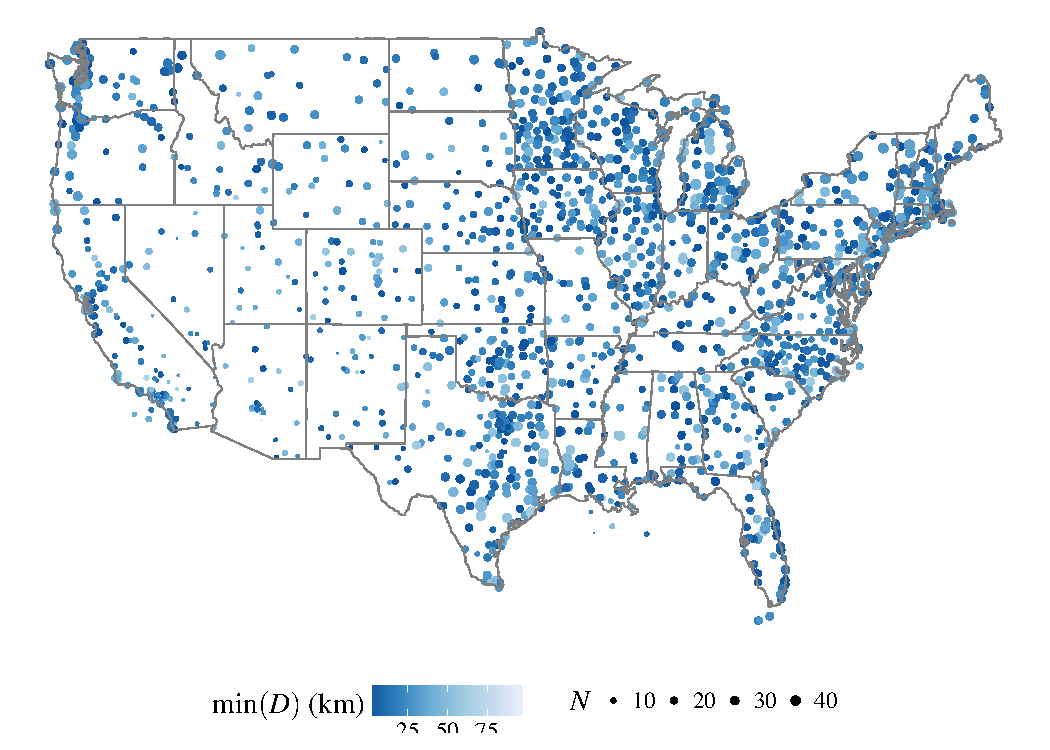
\includegraphics[width=0.95\textwidth]{figure/method-eval-asos-1} 

}



\end{knitrout}
  \caption{ASOS ceilometers used for CBASE CBH evaluation.  The size of the
    marker indicates the number of satellite--ceilometer CBH coincidences during
    the year 2007.  Color indicates the closest co-location distance achieved in
    2007.}
  \label{fig:asos}
\end{figure}

\begin{figure}
  \centering
  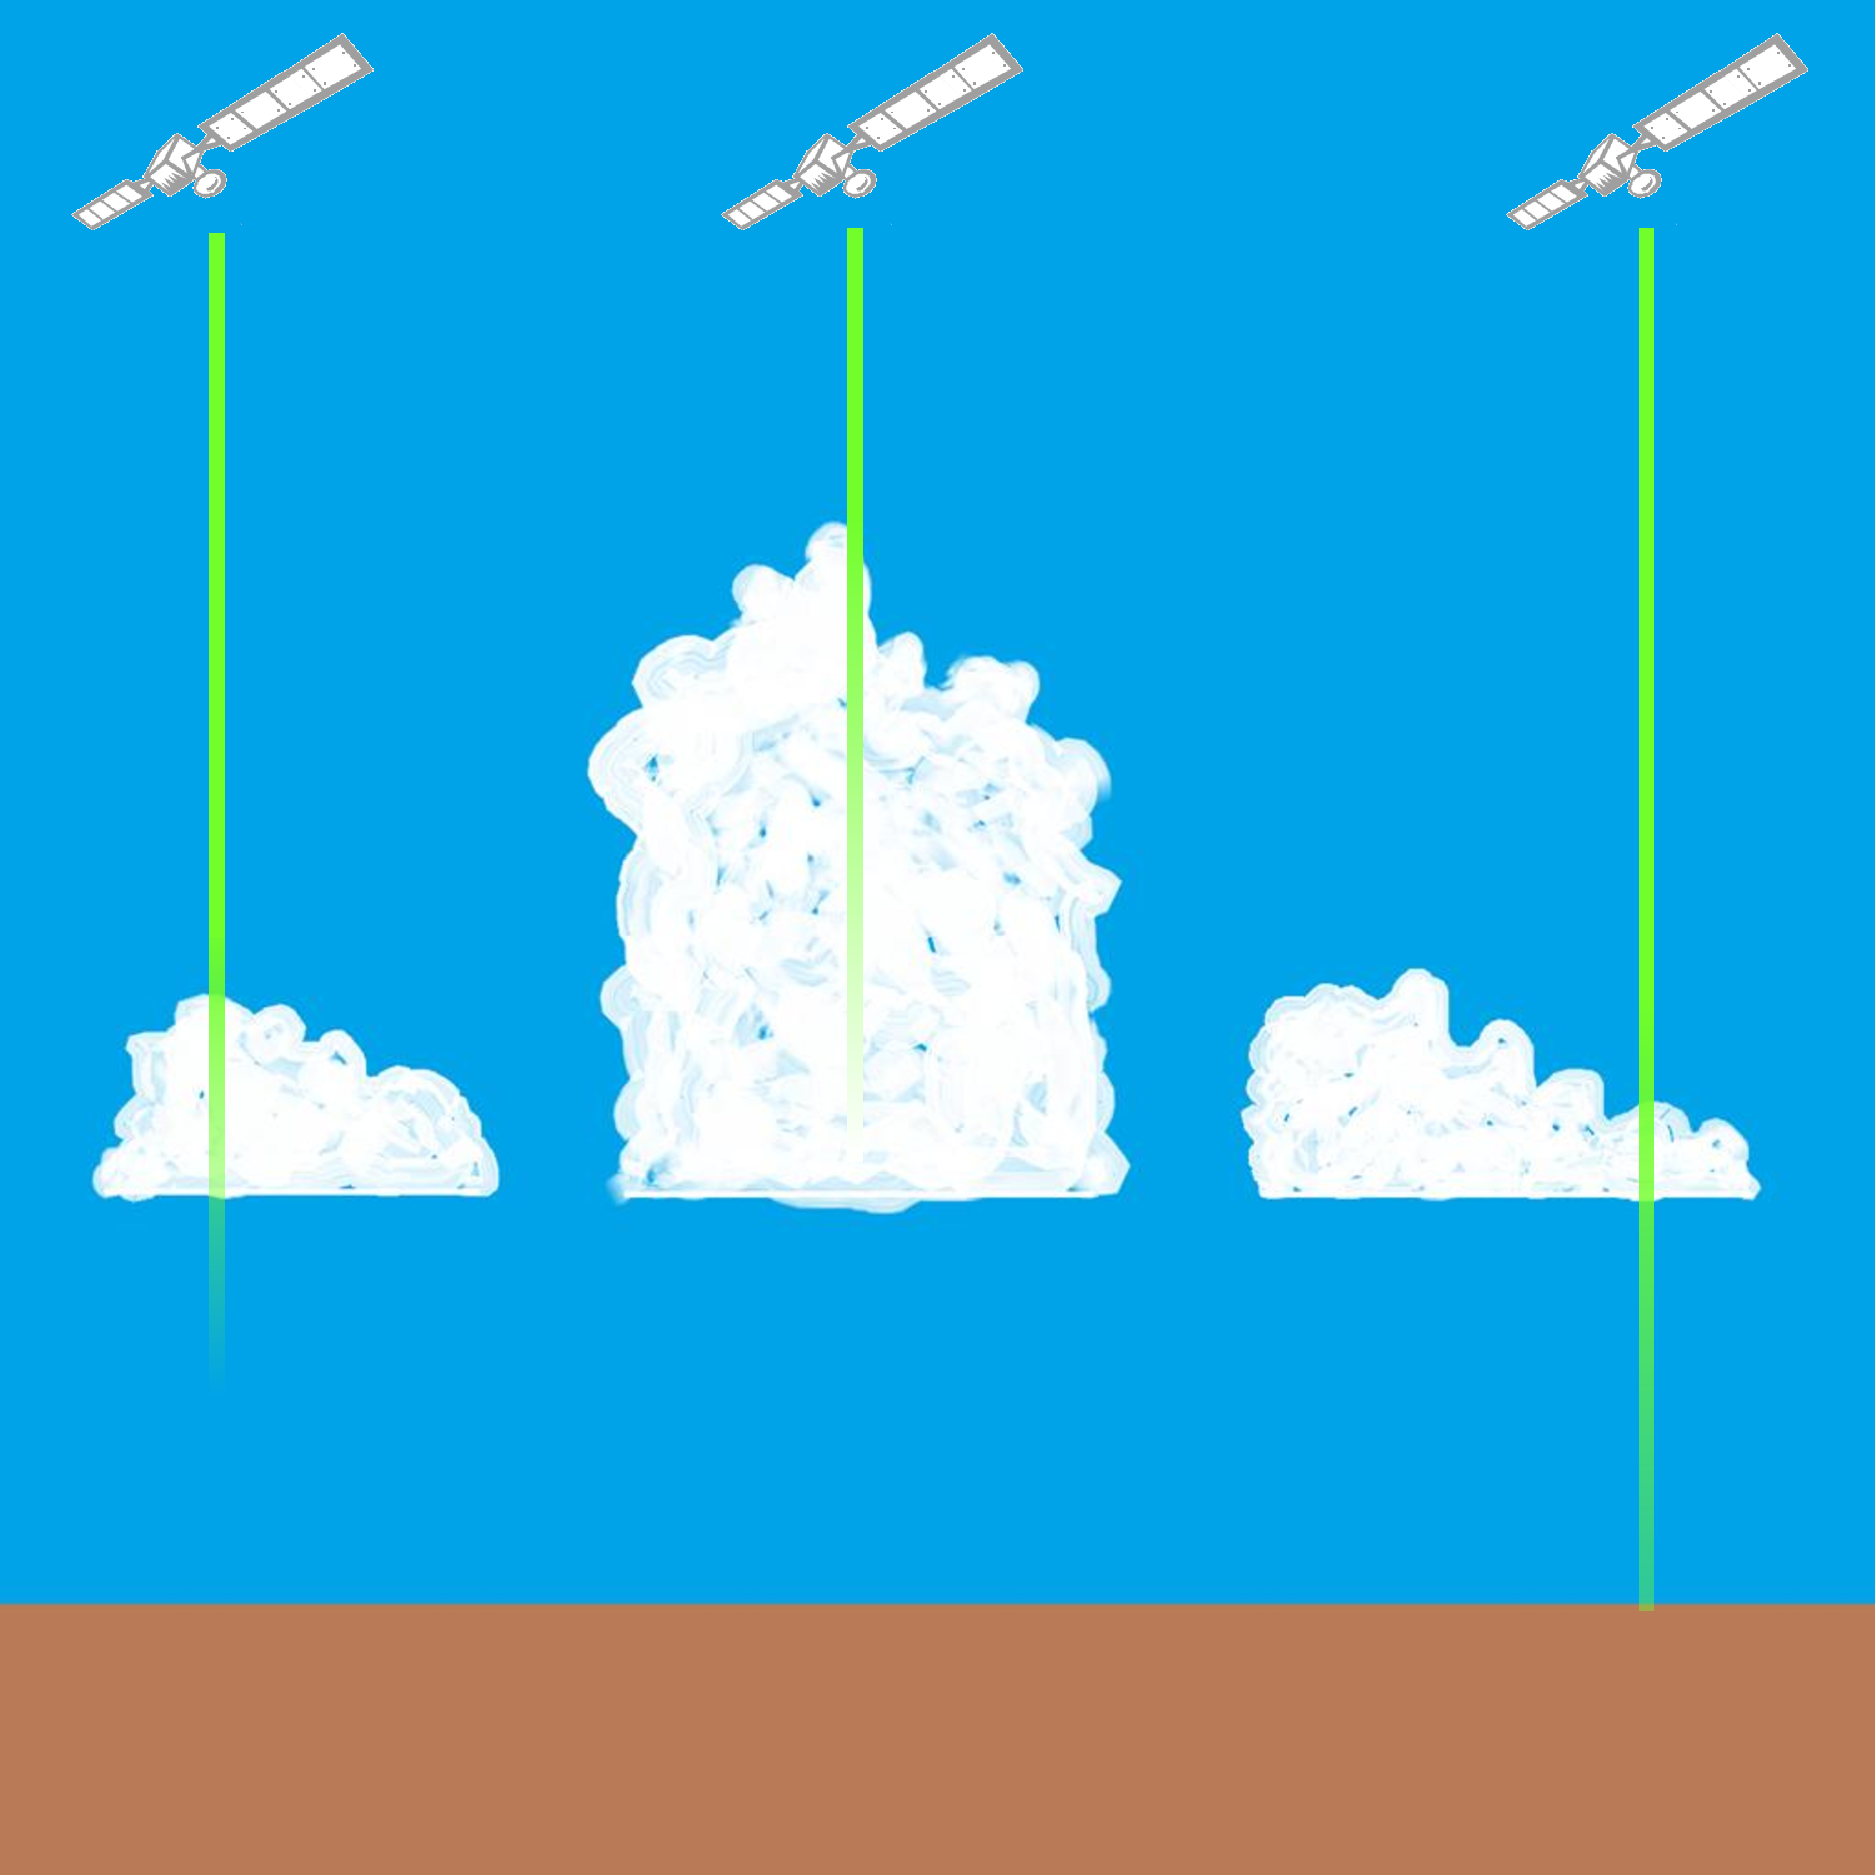
\includegraphics[width=0.5\linewidth,keepaspectratio=true]{CloudFieldCALIOP.pdf}
  \caption{Schematic of CALIOP cloud base determination and evaluation strategy.
    In optically thick clouds (left and center), the lidar attenuates
    significantly within the cloud, rendering the cloud base information
    unreliable.  However, the CBH of thin clouds (right) can be used as a proxy
    for thick clouds in a cloud field with homogeneous CBH.}
  \label{fig:method}
\end{figure}

\begin{figure*}
  \centering
\begin{knitrout}
\definecolor{shadecolor}{rgb}{0.969, 0.969, 0.969}\color{fgcolor}

{\centering 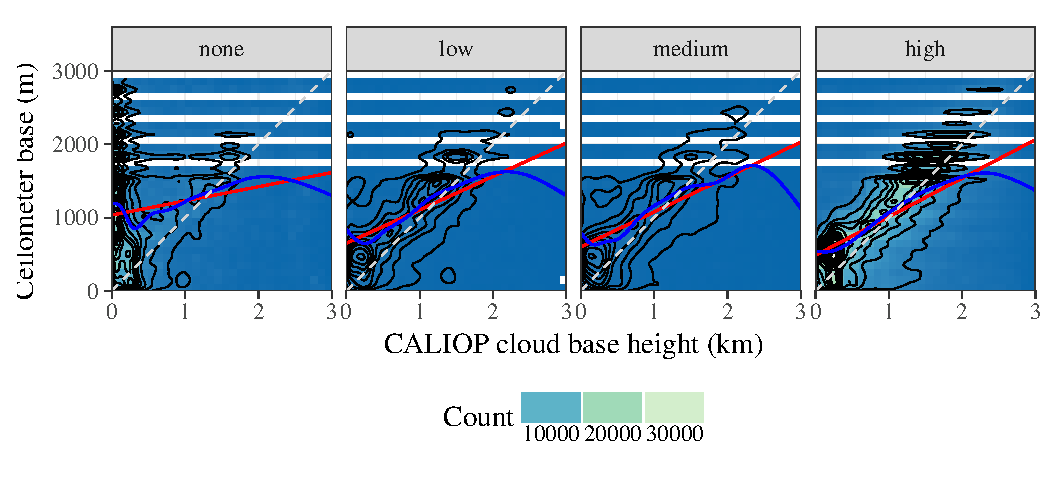
\includegraphics[width=0.95\textwidth]{figure/method-eval-qual-1} 

}



\end{knitrout}
  \caption{Scatter plots of CALIOP versus ceilometer local cloud base height
    faceted by the CALIOP VFM QA flag.  Color indicates the number of CALIOP
    profiles within each bin of ceilometer and CALIOP CBH; black
    lines are contours of the empirical joint probability density; the red line
    is a linear least-squares fit, with 95\% confidence interval shaded in light
    red; the blue line is a generalized additive model regression
    \citep{Wood2011}, with 95\% confidence interval shaded in light
    blue; the dashed gray line is the one-to-one line.  Statistics of the
    relationship between CALIOP and ceilometer base heights are provided in
    Table~\ref{tab:quality-qa}.}
  \label{fig:quality-qa}
\end{figure*}

\begin{table*}
  \centering
  \caption{Statistics of the relationship between ceilometer and CALIOP cloud
    base height faceted by CALIOP VFM QA flag.  Shown are the number of CALIOP
    profiles $n$, the product-moment correlation coefficient $r$ between CALIOP
    and ceilometer CBH, the RMSE, bias, and linear least-squares
    fit parameters.}
  \label{tab:quality-qa}
% latex table generated in R 3.4.2 by xtable 1.8-2 package
% Fri Oct 20 15:32:51 2017
\begin{tabular}{lrrrrl}
  \hline
\hline
feature.qa.lowest.cloud & $n$ & $r$ & RMSE (m) & bias (m) & fit \\ 
  \hline
none & 1410553 & 0.192 & $1.05 \times 10^{3}$ & $-$471. & $y = 0.193 x + \ensuremath{1.03 \times 10^{3}}$ m \\ 
  low & 301250 & 0.471 & 710. & $-$115. & $y = 0.456 x + 650.$ m \\ 
  medium & 212723 & 0.502 & 707. & $-$77.1 & $y = 0.476 x + 602.$ m \\ 
  high & 2877967 & 0.554 & 629. & 9.85 & $y = 0.526 x + 485.$ m \\ 
   \hline
\hline
\end{tabular}

\end{table*}

\begin{figure*}
  \centering
\begin{knitrout}
\definecolor{shadecolor}{rgb}{0.969, 0.969, 0.969}\color{fgcolor}

{\centering 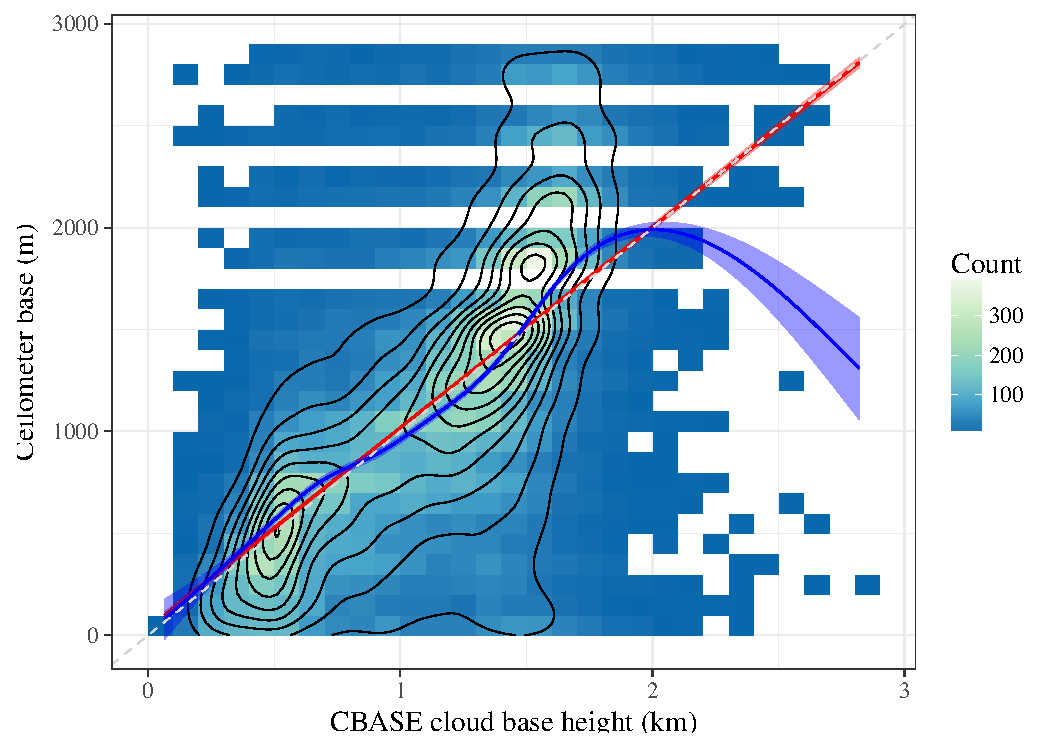
\includegraphics[width=0.95\textwidth]{figure/method-combo-plot-1} 

}



\end{knitrout}
  \caption{Scatter plot of CBASE versus ceilometer CBH for all A-Train
    overpasses over the CONUS available for 2007; for description of the
  plot elements, see Figure~\ref{fig:quality-qa}.  The linear fit has slope
  0.98 and intercept $33.96$~m.}
  \label{fig:eval}
\end{figure*}

\begin{figure}
  \centering
\begin{knitrout}
\definecolor{shadecolor}{rgb}{0.969, 0.969, 0.969}\color{fgcolor}

{\centering 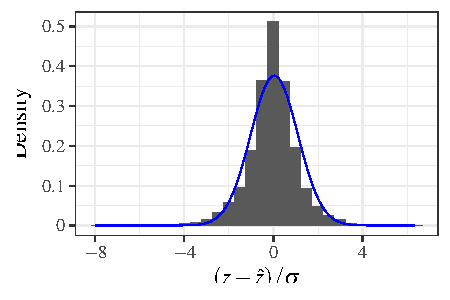
\includegraphics[width=0.5\textwidth]{figure/method-combo-eval-pull-1} 

}



\end{knitrout}
  \caption{Distribution function of cloud base error divided by predicted
    uncertainty; for the ideal case of unbiased CBH and unbiased
    uncertainty, the distribution would be Gaussian with zero mean and unit
    standard deviation.  The superimposed least-squares Gaussian fit (blue line)
    has mean 0.04 and
    standard deviation 1.06.}
  \label{fig:pull}
\end{figure}

% \begin{figure}
%   \centering
%   <<combo-eval-rmse,dev='tikz',fig.width=3,fig.height=2,out.width='0.5\\textwidth',message=FALSE,cache=FALSE,echo=FALSE>>=
%   @
%   \caption{Distribution of predicted CBH uncertainty.}
%   \label{fig:uncertainty}
% \end{figure}

%% \begin{figure*}
%%   \centering
%%   <<combo-plot-rmseclass,dev='tikz',fig.width=7,fig.height=5,out.width='0.95\\textwidth',message=FALSE,cache=FALSE,results='hide',echo=FALSE>>=
%%   @
%%   \caption{Scatter plot of CBASE versus ceilometer CBH for
%%     different classes of predicted uncertainty}
%%   \label{fig:rmseclass}
%% \end{figure*}

\begin{table*}[t]
  \centering
  \caption{CBASE cloud base statistics by decile of predicted uncertainty; see
    Table~\ref{tab:quality-qa} for a description of the 
    statistics provided.}
  \label{tab:rmseclass}

% latex table generated in R 3.4.2 by xtable 1.8-2 package
% Fri Oct 20 15:25:12 2017
\begin{tabular}{lrrrrl}
  \hline
\hline
pred.rmse & $n$ & $r$ & RMSE (m) & bias (m) & fit \\ 
  \hline
(167,427] & 2624 & 0.741 & 404. & $-$46.9 & $y = 1.03 x + 28.0$ m \\ 
  (427,453] & 2624 & 0.719 & 429. & $-$28.4 & $y = 1.06 x - 32.0$ m \\ 
  (453,469] & 2624 & 0.703 & 461. & $-$18.8 & $y = 1.09 x - 87.7$ m \\ 
  (469,484] & 2624 & 0.685 & 463. & $-$17.8 & $y = 1.03 x - 18.3$ m \\ 
  (484,497] & 2624 & 0.628 & 506. & $-$6.06 & $y = 0.976 x + 33.4$ m \\ 
  (497,508] & 2624 & 0.574 & 547. & $-$8.73 & $y = 0.986 x + 25.5$ m \\ 
  (508,522] & 2624 & 0.596 & 547. & $-$14.1 & $y = 1.01 x + 5.37$ m \\ 
  (522,541] & 2624 & 0.572 & 562. & $-$9.26 & $y = 0.967 x + 49.6$ m \\ 
  (541,573] & 2624 & 0.502 & 639. & $-$22.7 & $y = 0.939 x + 96.8$ m \\ 
  (573,748] & 2624 & 0.447 & 720. & 7.36 & $y = 0.829 x + 197.$ m \\ 
   \hline
\hline
\end{tabular}

\end{table*}



\begin{figure*}
  \centering
\begin{knitrout}
\definecolor{shadecolor}{rgb}{0.969, 0.969, 0.969}\color{fgcolor}

{\centering 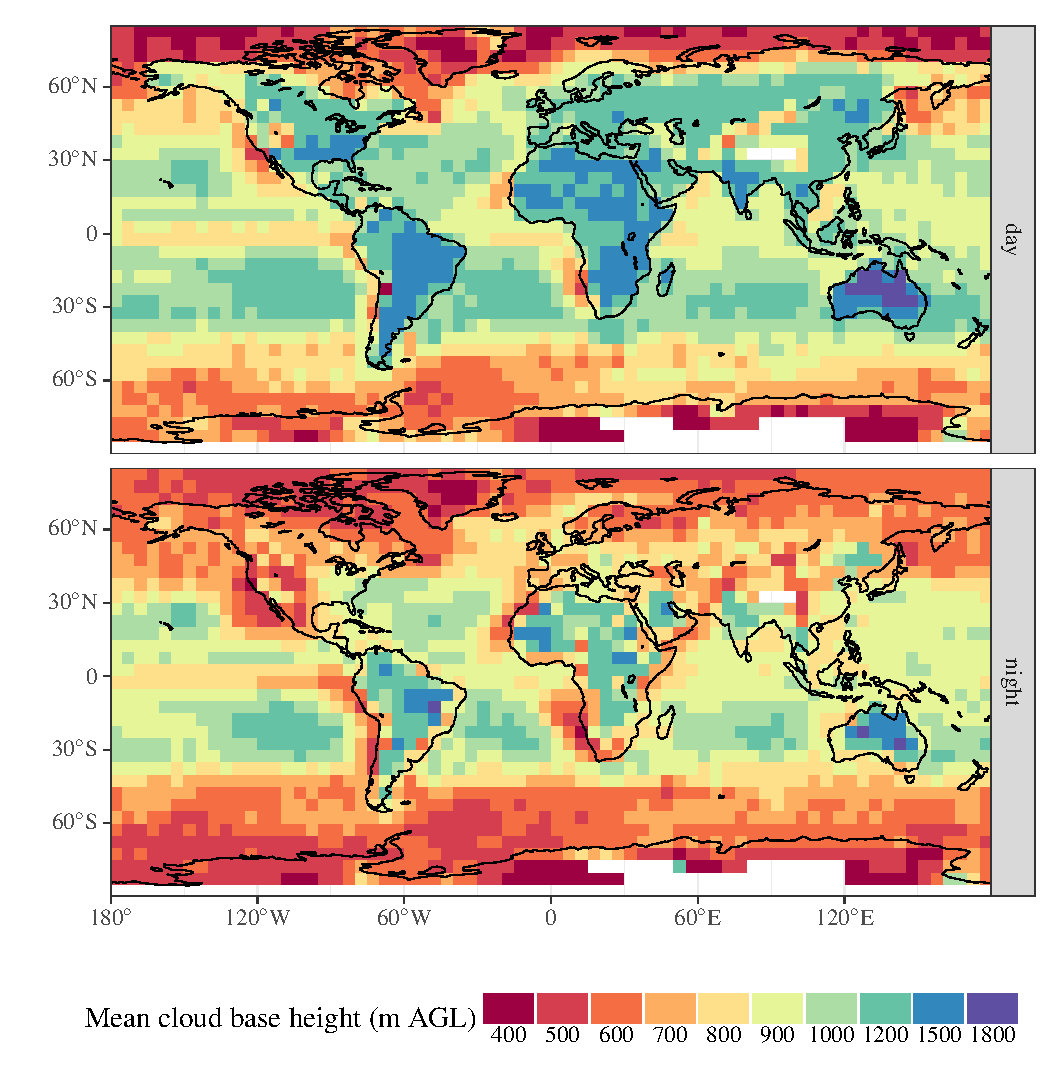
\includegraphics[width=0.95\textwidth]{figure/method-cbase-base-1} 

}



\end{knitrout}
  \caption{Geographic distribution of mean CBH above ground
    level.  Statistics are calculated within each $5\degree\times 5\degree$
    latitude--longitude box, and separately for CALIOP daytime (top) and
  nighttime (bottom)
    overpasses.}
  \label{fig:geo}
\end{figure*}

% \begin{figure*}
%   \centering
%   <<cbase-base-100,dev='tikz',fig.width=7,fig.height=7.2,out.width='0.95\\textwidth',message=FALSE,cache=FALSE,echo=FALSE,results='hide'>>=
%   vis.mean(cbase %>% filter(dist == 100), 14)
%   @
%   \caption{Geographic distribution of mean CBH above ground
%     level.  Statistics are calculated within each $5\degree\times 5\degree$
%     latitude--longitude box, and separately for CALIOP daytime and nighttime
%     overpasses ($D_\text{max} = 100$ km).}
%   \label{fig:geo}
% \end{figure*}

% \begin{figure*}
%   \centering
%   <<cbase-base-msl,dev='tikz',fig.width=7,fig.height=7.2,out.width='0.95\\textwidth',message=FALSE,cache=FALSE,echo=FALSE,results='hide'>>=
%   vis.mean(mutate(cbase, pred.ceilo = pred.ceilo.msl), 14)
%   @
%   \caption{Geographic distribution of mean CBH above sea level as a check that
%     the variable is correctly calculated}
%   \label{fig:geomsl}
% \end{figure*}

\begin{figure}
  \centering
\begin{knitrout}
\definecolor{shadecolor}{rgb}{0.969, 0.969, 0.969}\color{fgcolor}

{\centering 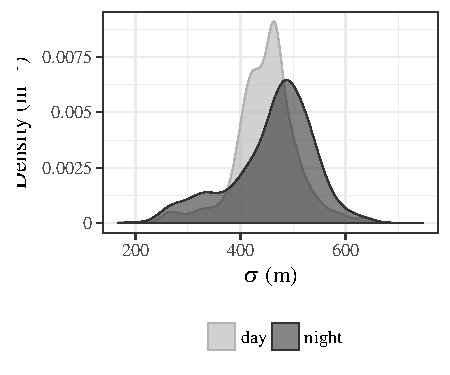
\includegraphics[width=0.5\textwidth]{figure/method-cbase-rmse-1} 

}



\end{knitrout}
  \caption{Distribution of predicted CBH uncertainty.}
  \label{fig:uncertainty}
\end{figure}

% \begin{figure}
%   \centering
%   <<cbase-rmse-100,dev='tikz',fig.width=3,fig.height=2.5,out.width='0.5\\textwidth',message=FALSE,cache=FALSE,echo=FALSE>>=
%   cbase %>% 
%   filter(dist == 100) %>%
%   ggplot(aes(x = pred.rmse, y = ..density.., fill = daynight, color = daynight)) + 
%   geom_density(alpha = 0.6, adjust = 5) + 
%   scale_fill_grey("", start = 0.7, end = 0.2) + 
%   scale_color_grey("", start = 0.7, end = 0.2) + 
%   labs(x = "$\\sigma$ (m)",
%        y = "Density (m$^{-1}$)") +
%   theme_bw() + theme(legend.position = "bottom")
%   @
%   \caption{Distribution of predicted CBH uncertainty ($D_\text{max} = 100$ km).}
%   \label{fig:uncertainty}
% \end{figure}

\begin{figure*}
  \centering
\begin{knitrout}
\definecolor{shadecolor}{rgb}{0.969, 0.969, 0.969}\color{fgcolor}

{\centering 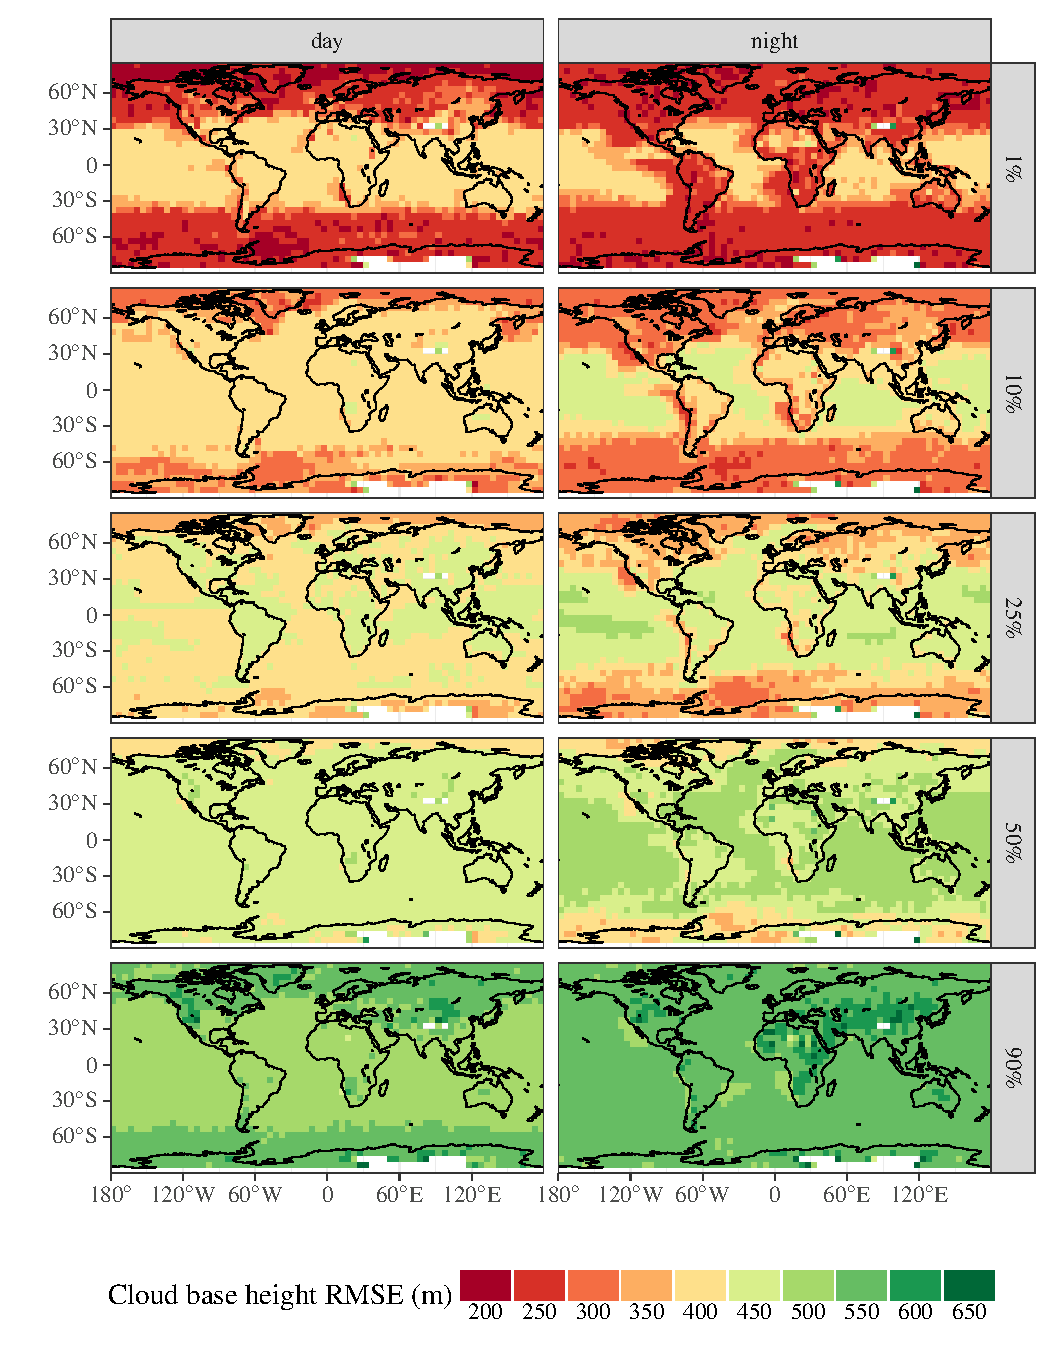
\includegraphics[width=0.95\textwidth]{figure/method-cbase-uncert-quantiles-1} 

}



\end{knitrout}
  \caption{Cloud base uncertainty quantiles.  Statistics are calculated within
    each $5\degree\times 5\degree$ latitude--longitude box.  The left (right)
    column shows statistics of daytime (nighttime) retrievals; daytime and
    nighttime are defined by the CALIOP VFM product.}
  \label{fig:uncert-quantiles}
\end{figure*}

% \begin{figure*}
%   \centering
%   <<cbase-uncert-quantiles-100,dev='tikz',fig.width=7,fig.height=9,out.width='0.95\\textwidth',message=FALSE,cache=FALSE,echo=FALSE,results='hide'>>=
%   vis.quantiles(cbase %>% filter(dist == 100), 14)
%   @
%   \caption{Cloud base uncertainty quantiles.  Statistics are calculated within
%     each $5\degree\times 5\degree$ latitude--longitude box.  The left (right)
%     column shows statistics of daytime (nighttime) retrievals; daytime and
%     nighttime are defined by the CALIOP VFM product ($D_\text{max} = 100$ km).}
%   \label{fig:uncert-quantiles}
% \end{figure*}

% \begin{figure*}
%   \centering
%   <<cbase-uncert-cdf,dev='tikz',fig.width=7,fig.height=9.5,out.width='0.95\\textwidth',message=FALSE,cache=FALSE,echo=FALSE,results='hide'>>=
%   vis.n(cbase, 14)
%   @
%   \caption{Cumulative distribution of cloud base uncertainty.  Statistics are
%     calculated within each $2\degree\times 2\degree$ latitude--longitude box.}
%   \label{fig:geo}
% \end{figure*}

\begin{figure*}
  \centering

\begin{knitrout}
\definecolor{shadecolor}{rgb}{0.969, 0.969, 0.969}\color{fgcolor}

{\centering 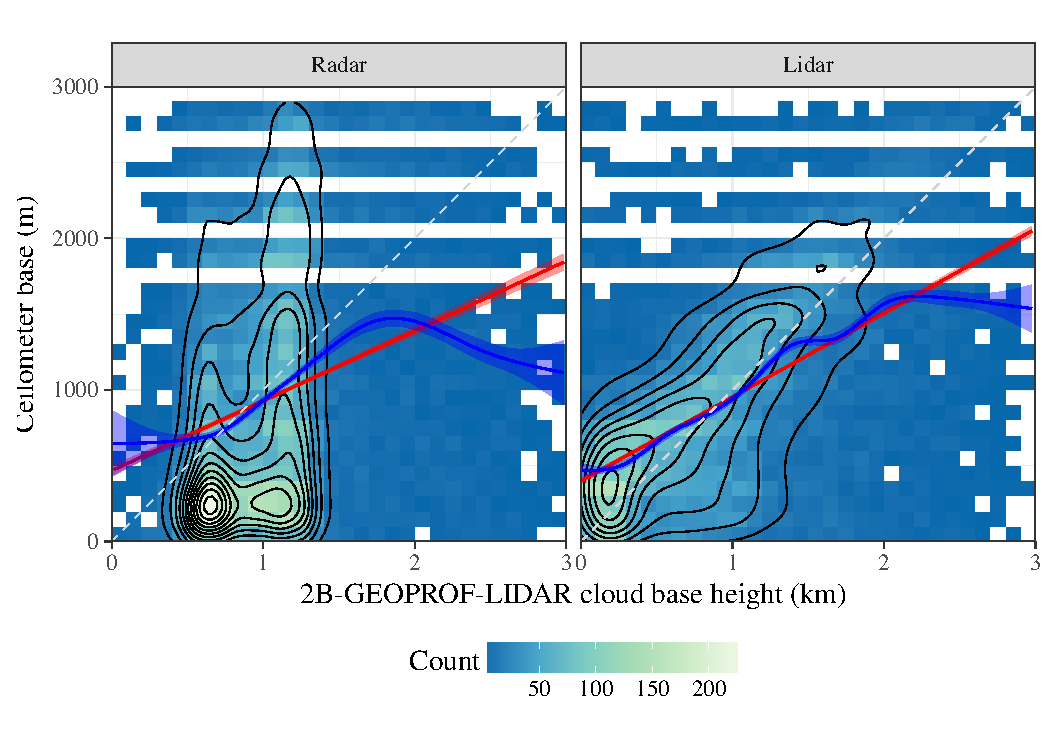
\includegraphics[width=0.95\textwidth]{figure/method-eval-2bgeoprof-1} 

}



\end{knitrout}
% latex table generated in R 3.4.2 by xtable 1.8-2 package
% Fri Oct 20 15:32:52 2017
\begin{tabular}{lrrrrl}
  \hline
\hline
flag.base & $n$ & $r$ & RMSE (m) & bias (m) & fit \\ 
  \hline
Radar & 15061 & 0.265 & 782. & 98.1 & $y = 0.461 x + 466.$ m \\ 
  Lidar & 12813 & 0.564 & 594. & 16.3 & $y = 0.555 x + 399.$ m \\ 
   \hline
\hline
\end{tabular}

  \caption{Scatter plot of 2B-GEOPROF-LIDAR versus ceilometer CBH
    faceted by the source of the cloud base (radar-only or lidar-only; due to
    their rare occurrence, combined radar--lidar base heights are not shown).
    For description of the plot elements, see Figure~\ref{fig:quality-qa}.  Statistics of the
    relationship between 2B-GEOPROF-LIDAR and ceilometer base heights are provided in
    Table~\ref{tab:2bgeoprof}.}
  \label{fig:eval-2b}
\end{figure*}

\begin{table*}
  \caption{Statistics of the relationship between ceilometer and
    2B-GEOPROF-LIDAR CBH; see Table~\ref{tab:quality-qa} for a
    description of the statistics provided.}
  \label{tab:2bgeoprof}
  \centering
% latex table generated in R 3.4.2 by xtable 1.8-2 package
% Fri Oct 20 15:32:52 2017
\begin{tabular}{lrrrrl}
  \hline
\hline
flag.base & $n$ & $r$ & RMSE (m) & bias (m) & fit \\ 
  \hline
Radar & 15061 & 0.265 & 782. & 98.1 & $y = 0.461 x + 466.$ m \\ 
  Lidar & 12813 & 0.564 & 594. & 16.3 & $y = 0.555 x + 399.$ m \\ 
   \hline
\hline
\end{tabular}

\end{table*}



\end{document}
